\section{Algorithms of construction of gadgets}
\label{sec:search}

Let $f: \B^\ell \mapsto \B$ a Boolean function with $\ell$ entries. This section addresses the problem of constructing a gadget for $f$. To do so, we pick a value for $p$ and we search a vector of $\ell$ $p$-encodings $\Vec{\Encoding_{in}}$ suitable for $f$. 

\subsection{Reduction of the Search Space}
\label{sec:restriction}

While exhaustive search is a first option, it quickly becomes impractical due to the explosion of the number of possibilities as $p$ grows. As a consequence, a reduction of the search space is needed without leaving out a potential solution.

We introduce two lemmas that will be used to reduce the search space:

\begin{lemma} [Reducibility to singletons]
    Let $f: \B^\ell \longrightarrow \B$ and let $(\Encoding_1, \dots, \Encoding_l)$ be a vector of $p$-encodings suitable for $f$ and having the form:
    $\forall~i \in \{1, \dots, \ell\}, \Encoding_i = \EncDef{\{x_j^{(i)}\}_{1 \le j \le l_0^{(i)}}}{\{y_j^{(i)}\}_{1 \le j \le l_1^{(i)}}}$.
    Then any vector of canonical $p$-encodings $(\Encoding'_1, \dots, \Encoding'_l)$ of the form: $ \forall~i \in \{1, \dots, \ell\}, \Encoding'_i = \EncDef{\{x^{(i)}\}}{\{y^{(i)}\}}$ with $x^{(i)} \in \Encoding_i(0)$ and $ y^{(i)} \in \Encoding_i(1)$ is suitable for the function $f$ as well.
    \label{lemma:reduction}
\end{lemma}


\begin{proof}
Let us assume that the vector $\Encoding = (\Encoding_1, \dots, \Encoding_l)$ of Lemma \ref{lemma:reduction} is suitable for the function $f$. Then the sets $\mathcal{P}_0$ and $\mathcal{P}_1$ constructed like in Equation \ref{def:sets_p} are disjoint.
Now, let us consider the vector of canonical $p$-encodings $\Encoding' = (\Encoding'_1, \dots, \Encoding'_l)$ respecting the property:
$$
\forall~b \ \in \B, \forall 
~i \in \{0, \dots, \ell\}, \Encoding'_i(b) \subset \Encoding_i(b).
$$
As a consequence, if we build the sets $\mathcal{P'}_0$ and $\mathcal{P'}_1$ relative to the encodings $\Encoding'$, then we naturally get $\mathcal{P'}_0 \subset \mathcal{P}_0$ and $\mathcal{P'}_1 \subset \mathcal{P}_1$. So we get $\mathcal{P'}_0 \cap \mathcal{P'}_1 = \emptyset$, proving Lemma \ref{lemma:reduction}.
\end{proof}


\begin{lemma}[Reducibility to the singleton zero]
    Let $f: \B^\ell \longrightarrow \B$ and let $(\Encoding_1, \dots, \Encoding_l)$ be a vector of $p$-encodings suitable for $f$ and of the form: $\forall i \in \{1, \dots, \ell\}, \Encoding_i = \EncDef{\{x^{(i)}\}}{\{y^{(i)}\}}$
    Then any vector of canonical $p$-encodings $(\Encoding'_1, \dots, \Encoding'_l)$ of the form: $\forall~i \in \{1, \dots, \ell\}, \Encoding'_i = \EncDefOne{y^{(i)} - x^{(i)}}$
    is suitable for the function $f$ as well.
    \label{lemma:enczero}
\end{lemma}


\begin{proof}
Let $f: \B^\ell \longrightarrow \B$ be a function and $\Encoding$ be a vector of canonical $p$-encodings $(\Encoding_1, \dots, \Encoding_l)$ suitable for $f$ with:
$$
\forall~i \in \{1, \dots, \ell\}, \Encoding_i = \EncDef{\{x^{(i)}\}}{\{y^{(i)}\}}.
$$
Let us build the sets $\mathcal{P}_0$ and $\mathcal{P}_1$ according to Equation \ref{def:sets_p}. Each element of these sets is the sum of exactly one element of each $p$-encoding, that is to say an element $\Encoding_i(0) \cup \Encoding_i(1)$.

Let us pick an indice $k \in \{1, \dots, \ell\}$, a value $a \in \Z_p$ and replace $\Encoding_k$ in the vector $\Encoding$ by: 
$$
\Encoding'_k = \EncDef{\{x^{(i)} - a\}}{\{y^{(i)} - a\}}
$$

By using the Property \ref{prop:sum_constant}, we directly have $\mathcal{P}'_0 \cap \mathcal{P}'_1 = \emptyset$ from $\mathcal{P}_0 \cap \mathcal{P}_1 = \emptyset$ (by suitability of the encodings for $f$).

By iterating this procedure on each of the $\ell$ elements of $\Encoding$, and by picking each time $a = -x^{(i)}$, we prove Lemma \ref{lemma:enczero}.
\end{proof}



Using both Lemmas \ref{lemma:reduction} and \ref{lemma:enczero}, we can restrict the search to the encodings of the form $$\Encoding_i = \EncDefOne{d_i}$$ with $d_i \ne 0$ without any loss of generality. 


Moreover, we restrict the solution further: we only consider $p$-encodings with $p$ \emph{odd} and \emph{prime}. The choice of an odd $p$ allows to free ourselves from the negacyclicity constraint (more about that in Section \ref{sec:solving_negacyclicity}). To explain the constraint of primality, we introduce the following lemma, that allows to drastically improve the performances of the search:

\begin{lemma}
    Let $p$ be a prime and $f:\B \longrightarrow \B$ be a Boolean function and let $\Encoding = (\Encoding_1, \dots, \Encoding_l)$ be $p$-encodings suitable for $f$ with: $\forall~i \in \{1, \dots, \ell\}, \Encoding_i = \EncDef{\{x^{(i)}\}}{\{y^{(i)}\}}$. For every $a \in \Z_p \setminus \{0\}$, the vector of $p$-encodings $\Encoding '= (\Encoding'_1, \dots, \Encoding'_l)$ with: $\Encoding'_i = \EncDef{\{[a \cdot x^{(i)}]_p\}}{\{[a \cdot y^{(i)}]_p\}}$
    is suitable for $f$ as well.
    \label{lemma:multiplication_in_prime_group}
\end{lemma}

\begin{proof}
This is an immediate consequence of Property \ref{prop:mult_constant}.
\end{proof}

As a consequence, if $p$ is prime (which we shall always choose in practice), any solution can be turned into a solution with $d_1 = 1$ by simply multiplying all the $p$-encodings of the solution by $[d_1^{-1}]_p$. So we can fix $d_1 = 1$ without any loss of generality, reducing drastically the size of the search space. 





\subsection{Formalization of the Search Problem}

According to the lemmas from Section \ref{sec:restriction}, we can reduce the problem of finding a vector of $p$-encodings $(\Encoding_1, \dots, \Encoding_l)$ such that $f(\Encoding_1, \dots, \Encoding_l)$ is valid to the problem of finding a vector $\vec{d} = (d_1, \dots, d_l)$ such that $\Encoding_i = \EncDefOne{d_i}$ and $f(\Encoding_1, \dots, \Encoding_l)$ is valid. In the following, we describe an algorithm to find such a vector $\vec d$.


We denote $V$ the matrix of elements of $\B$ of shape $2^\ell \times \ell$ gathering all the possible sequences of entries for the function $f$:

$$V = \left ( \begin{matrix}
0 & \dots & 0 & 0\\
0 & \dots & 0 & 1\\
\vdots & \ddots & \vdots & \vdots\\
1 & \dots & 1 & 1
\end{matrix}
\right ) $$

Also, we denote by $\Vec{b}$ the vector of all the outputs of the function $f$, sorted in same order as the rows of $V$. Thus, we have: $\forall~i \in \{1, \dots, 2^\ell\}, b_i = f(V_i)$
for $V_i$ the $i$th row of $V$. Let us define the vector $\vec r$ as: $\Vec{r} = V \vec{d}$. To make $\vec d$ a solution of the problem, $\vec r$ has to verify the following property:
\[
\forall~i, j \in \{1, \dots, 2^\ell\}^2, f(V_i) \neq f(V_j) \implies r_i \neq r_j   
\]
An alternative formulation is: we look for two disjoint subsets $\mathcal{P}_0$ and $\mathcal{P}_1$ of $\Z_p$, such that: $f(V_i) = b \Longleftrightarrow r_i \in \mathcal P_b$.

The following section describes an algorithm finding a solution to this problem.

\subsection{Algorithm}
\label{sec:search_algorithm}

We start by constructing two sets $\mathcal F$ and $\mathcal T$ such that: \[\mathcal F = \{V_i \vert b_i = 0\} \text{ and } \mathcal T = \{V_i \vert b_i = 1\}.\]
Each line $V_i$ represents a linear combination of the $d_j$'s, that verifies:
\[r_i = \sum_{j=0}^{\ell} V_{ij} \cdot d_j \mod p.\]
The values $r_i$ produced by the elements of $\mathcal{F}$ must be different from the ones produced by $\mathcal{T}$. As a consequence, we can write:
\[\forall~(V_i, V_j) \in \mathcal F \times \mathcal T, \sum_{k=0}^\ell V_{ik} \cdot d_k \neq \sum_{k=0}^\ell V_{jk} \cdot d_k,\] which is equivalent to writing:
\[\forall~(V_i, V_j) \in \mathcal F \times \mathcal T, \sum_{k=0}^\ell (V_{ik} - V_{jk}) \cdot d_k \neq 0.\]
So we can rewrite our constraints in the set $\mathcal C =  \{V_i - V_j \vert (V_i, V_j) \in \mathcal F \times \mathcal T\}.$ $\mathcal{C}$ contains vectors with coordinates in $\{0, 1, -1\}$ representing linear combinations that have to be non-zero. Note that if an element of the set $\mathcal{C}$ is the opposite of an other, it does not bring further constraint and can thus be safely discarded from the set.

The use of a set in the implementation at this point of the algorithm allows to remove a lot of duplicate constraints and to simplify the next step. Then, the problem reduces to solving a ``linear system of inequalities'' in the ring $\Z_p$: 

$$
\begin{cases}
    c_1^{(1)} \cdot d_1 + \dots + c_l^{(1)} \cdot d_l \ne 0 \mod p \\
    c_1^{(2)} \cdot d_1 + \dots + c_l^{(2)} \cdot d_l \ne 0 \mod p\\
    \vdots
\end{cases} \text{ with }
c_i^{(j)} \in \{0, \pm 1\}
$$


After filtering, we pack all the elements of $\mathcal{C}$ in $\ell$ matrices $\{C_i\}_{1 \le i \le \ell}$ (each row being a linear combination), where the matrix $C_i$ packs all the constraints involving only the $i$ first inputs (i.e. all the coefficients of column index greater than $i$ are zeros).


We then perform a recursive search (Algorithm \ref{alg:add_element}), affecting at each step of depth $i$ a possible value $d_i$ for the $i$-th input. To do so, we call Algorithm \ref{alg:get_possible_values} to construct the set of all possible values complying with the constraints of the matrix $C_i$ and the previously set values for the preceding inputs. If we reach a dead-end, we backtrack by deleting the preceding input and assigning it the next possible value. Algorithms \ref{alg:add_element} and \ref{alg:get_possible_values} formalize this idea: Algorithm \ref{alg:add_element} is a  basic recursive backtracking algorithm using calls to the set construction function (Algorithm \ref{alg:get_possible_values}) to get the possibilities for the next value of $\vec{d}$. The latter, when called at depth $j+1$, takes as input the 
$j$ values already computed at higher depth for $\vec{d}$ and the matrix of constraints $C_{j+1}$. Each line of $C_{j+1}$ creates a (potentially duplicate) forbidden value for $d_{j+1}$, these values are all computed and the complement of this set in $\Z_p$ is returned by the algorithm (i.e. the set for possible values for $d_{j+1}$ at this point of the search).

\begin{theorem}
     Running Algorithm \ref{alg:add_element} with increasing values of $p$ ensures that the first solution $\vec d$ found is optimal for the function $f$, i.e. the solution works and its associated $p$ is the smallest as possible.   
\end{theorem}


\begin{algorithm}
	\caption{Recursive function \texttt{search} that adds an element to the vector $\vec{d}$}
	\label{alg:add_element}
	
	\KwIn{
		$\left\{
		\begin{aligned}
			&\vec{d} = (d_i)_{1 \le i \le j}  \text{: vector of values already computed} \\
			&\vec{\mat{C}} = \{ \mat{C}_i \mid i \in \{0, \dots, \ell-1\} \} \text{: pre-computed constraint matrices} \\
			&p \in \mathbb{N}^* \text{: modulus of the input encodings} \\
			&\ell \in \mathbb{N}^* \text{: target number of encodings required}
		\end{aligned}
		\right.$
	}
	
	\KwResult{
		$\vec{d}$: \text{a list of encodings such that $f$ is evaluable}
	}
	
		% Add vertical space and horizontal line
	\vspace{0.5em} % adjust the space as needed
	\hrule
	\vspace{0.5em} % adjust the space as needed
	
	
	
	\uIf{$j = \ell$}{
		\Return{$\vec{d}$} \Comment*[r]{Base case: full solution found}
	}
	\Else{
		$\mathcal{P} \gets \texttt{get\_possible\_values}(\vec{d}, \mat{C}_{j+1}, p)$ \Comment*[r]{Compute possible values for $d_k$}
		\For{$x \in \mathcal{P}$}{
			$\vec{d} \gets (\vec{d} \,\|\, x)$ \Comment*[r]{Append $x$ to current vector}
			$\vec{d}_{\text{sol}} \gets \texttt{search}(\vec{d}, \vec{\mat{C}}, p, \ell)$ \Comment*[r]{Recursive call}
			\uIf{$\vec{d}_{\text{sol}} \ne \bot$}{
				\Return{$\vec{d}_{\text{sol}}$} \Comment*[r]{Propagate valid solution}
			}
			\Else{
				$\vec{d} \gets \vec{d}[:j+1]$ \Comment*[r]{Backtrack by removing $x$ from the solution vector}
			}
		}
		\Return{$\bot$} \Comment*[r]{All possibilities failed}
	}
	
\end{algorithm}



\begin{algorithm}
	\caption{Function \texttt{get\_possible\_values} that builds the set of possible values for the next slot of $\vec{d}$ given the slots already filled in.}
	\label{alg:get_possible_values}
	
	\KwIn{
		$\left\{
		\begin{aligned}
		    &\vec{d}:= (d_i)_{\{1 \le i \le j\}}  \text{ :the set of values for the inputs already computed}\\
		    &\mat{C}_{j + 1}   \text{ :The matrix of constraints of this step, pre-computed}\\
			&p \in \N^* \text{: the modulus of input encoding}
		\end{aligned}
		\right.$
	}
	
	\KwResult{
		$S$ : contains only values suitable for the $j+1$-th slot of $\vec{d}$.
	}
	
	
	% Add vertical space and horizontal line
	\vspace{0.5em} % adjust the space as needed
	\hrule
	\vspace{0.5em} % adjust the space as needed
	
	$\bar S \gets \{\}$ \Comment*[r]{$\bar S$ is the set of forbidden values for $d_{j+1}$}
	
	\For {$c \in C_{j+1}$}{
	  	$\bar c \gets (- c[-1] \cdot c[0], -c[-1] \cdot c[1], \dots)$ \Comment*[r]{}
		$\bar C \gets \bar C \cup \{\bar c\}$ \;
	    $\bar c \gets c[j+1]$ \Comment*[r]{We retrieve the $(j+1)$th coefficient of the inequation $c$}
	    $\bar S \gets \bar S \cup \left \{\modulo{- \bar c \cdot \sum_{k=1}^{j} c_k \cdot d_k}{p} \right \}$ \Comment*[r]{We compute the value forbidden by $c$}	
	
	}
	$S \gets \Z_p \setminus \bar S$\\
	\Return{$S$}
\end{algorithm}









\paragraph{Optimizations:} Several optimizations are possible to improve the performances of the search. First, in Algorithm \ref{alg:get_possible_values}, one can check the size of the set $\bar S$ at each iteration and stop as soon as the size of the set is $p$. Such a set means that a dead-end has been reached and that no value will be returned by the function. Then, one can leverage symmetries existing in the table but also in the function. For example, if we consider the function $f: (x, y) \longrightarrow x \oplus y$, the two variables $x$ and $y$ have symmetric roles. Thus, if the pair of encodings $(\Encoding_x, \Encoding_y)$ is valid, then the pair $(\Encoding_y, \Encoding_x)$ is valid as well. As a consequence, one can arbitrarily set $d_x \le d_y$ and removing half the possibilities for $(x, y)$.




\paragraph{Development of an heuristic:} This algorithm of the previous section is deterministic and finds any existing set of encodings compliant with the function $f$ \emph{for a given value of $p$}. However, the right value for $p$ is not known \emph{a priori}, so we have to run the full algorithm for each possible value of $p$ until we find one that works. For these reasons, we might prefer an efficient heuristic over the previous algorithm in some contexts. In Section \ref{sec:heuristic_matthieu}, we define such a heuristic which allows to drastically improve the performance by executing directly the algorithm with realistic values for $p$. 




\subsection{Performances measurements}

In this section, we present some experimental results to demonstrate the performances of the algorithm. We ran Algorithm \ref{alg:add_element} for a lot of random Boolean functions of arity $\ell$. Two metrics are particularly interesting for us:
\begin{itemize}
    \item The running time of the algorithm, especially in the cases where there is no solution.
    \item The probability of success, for a random function
\end{itemize}


Figure \ref{fig:heatmap_success} shows the rate of success for random Boolean functions of arity $\ell \in \{2, 9\}$ and for prime values of $p \in [3, 39]$. It illustrates the intuitive idea that one has to increase $p$ to evaluate functions of bigger arity $\ell$. It also give a rough idea of the value of $p$ required for a given function of arity $\ell$.

\begin{figure}
    \centering
    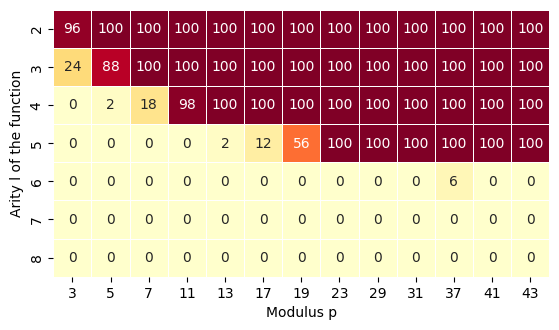
\includegraphics[]{img/p_encodings/heatmap_success.png}
    \caption{Rate of success of the algorithm for 100 random Boolean functions for different values of $\ell$ and $p$.}
    \label{fig:heatmap_success}
\end{figure}


Figure \ref{fig:lineplot_timings} shows the evolution of the time of execution of the algorithm for random Boolean functions \emph{for which no solution exists}.  It shows the explosion of the complexity for high values of
$p$, and justifies the need of a more efficient algorithm for those function (we introduce one in Section \ref{sec:graphs}).  


\TODO{Harmoniser l'algorithme suivant (commenté)}
\begin{figure}
    \centering
    \begin{minipage}{0.55\textwidth}
        \centering
        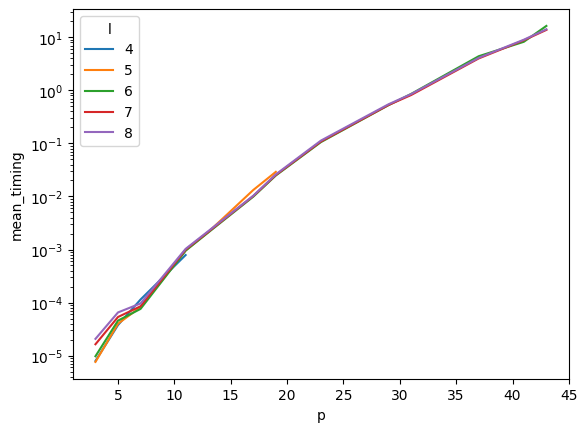
\includegraphics[width=\linewidth]{img/p_encodings/lineplot_timings.png}
        \caption{Running time of the algorithm for different values of $\ell$ and $p$ for random functions. Note that the scale is logarithmic.}        
        \label{fig:lineplot_timings}
        \end{minipage}\hspace{0.04\textwidth}
    \begin{minipage}{0.35\textwidth}
        \centering
        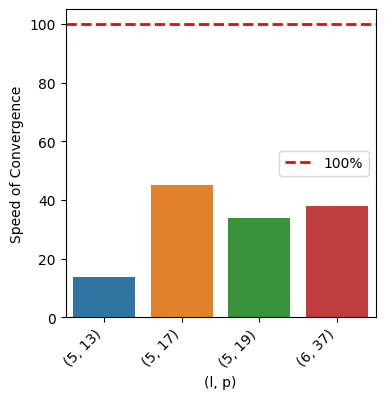
\includegraphics[width=\linewidth]{img/p_encodings/barplot.png}
        \caption{Ratio between the time to find a solution when it exists with the time to run the full algorithm when no solution exists.}
        \label{fig:barplot_ratio}
    \end{minipage}
    \caption{Some metrics about running time.}
    \label{fig:overall}
\end{figure}
Lastly, Figure \ref{fig:barplot_ratio} shows how long it takes to find a solution when one exists, relatively to the running time when no solution exist at all. It illustrates a form of "speed of convergence" and shows that it is located around $\frac{1}{3}$.



    
\subsection{An Efficient Sieving Heuristic to Find Suitable Encodings}
\label{sec:heuristic_matthieu}


Let us consider a function $f: \B^\ell \mapsto \B$ of matrix of constraints $C=(C_j^{(i)})_{\substack{1 \le i \le n_j\\1 \le j \le \ell}}$ and its associated system of linear inequalities:

$$
\left \{
\begin{array}{c}
     c_1^{(1)} \times d_1 + c_2^{(1)} \times d_2 + \dots + c_\ell^{(1)} \times d_\ell   \neq 0 \mod p\\
     c_1^{(2)} \times d_1 + c_2^{(2)} \times d_2 + \dots + c_\ell^{(2)} \times d_\ell \neq 0 \mod p\\
    \dots
\end{array}
\right .
$$


The principle is to sample random values in $\Z$ (with some large bound) and affect them to the $d_j$'s. If all the corresponding values for all the $C_i = \sum_{j=1}^{\ell} c_j^{(i)} \times d_j$ are not divisible by a value $p$, then the vector $(d_j \mod p \mid j \in \{1, \dots, \ell\})$ is a solution of the system of inequalities generated by $C$. 


To reduce the amount of samples required to find a solution, we want to avoid sampling trivially wrong sets of $d_j$'s. For example, if all the $d_j$'s are themselves divisible by $p$, then the $C_i$'s will all be divisible as well. To tackle this problem, we perform the sampling across \emph{prime numbers in $\Z$}.



\begin{algorithm}
	 \caption{Sample a solution $\vec d$ in $\Z$ for a function $f$ and returns a possible value for $p$.}
	\label{alg:heuristic_matthieu}
	
	\KwIn{
		$\left\{
		\begin{aligned}
				&\{\mat{C}_i\}_{1 \le i \le n} \text{: The lines of the matrix of constraints $\mat C$ of the function $f$ }\\
			    &P \text{: The set of possible values for $p$ to be tested}\\
			    &D \text{: The set of possible values in $\Z$ to assign to the $d_i$'s. (large primes)}
		\end{aligned}
		\right.$
	}
	
	\KwResult{
 		$p$ such that it is possible to evaluate $f$ using a modulus smaller or equal than $p$.
	}
	
	
	% Add vertical space and horizontal line
	\vspace{0.5em} % adjust the space as needed
	\hrule
	\vspace{0.5em} % adjust the space as needed
	
	$\vec{d} \drawfrom D$ \Comment*[r]{Sample random prime values in $\Z$}
	$\vec r = C \times \vec{d}$  \Comment*[r]{$\vec r$ is the right member of the system}
	\For {$p \in P$}{
	    \uIf{$0 \in [\Vec{r}]_p$}{
	        $P \gets P \setminus \{p\}$ \Comment*[r]{If this value of $p$ divides one of the coordinates of $\vec r$, then it will not work}
		}
	}
	\uIf{$\mid P \mid > 0$}{
	  \Return{$\min(P)$} \Comment*[r]{Returns the smallest possible value for $p$, if any.}
	 }
	
	\Return{$\bot$}	
\end{algorithm}

\TODO{Harmoniser ci-dessus}

Running this algorithm several times and keeping the smallest returned value for $p$, one gets an upper bound on the minimum $p$ required to evaluate a function with our framework. Note that, on the contrary of the deterministic search algorithm, this heuristic does not require a prime $p$.


\paragraph{Example:} Let us consider the s-box of the block cipher ASCON. We study this s-box in more details and provide an exact optimized solution for its homomorphic evaluation in Section \ref{sec:ascon}. Here, we apply Algorithm \ref{alg:heuristic_matthieu} on the five functions generating the five output bits and monitor the results until we gather $N=10000$ non-zero possible values for $p$.


The figure \ref{fig:ascon_0_p_frequencies} shows the repartition of the returned values of $p$ by the algorithm during these $N$ runs on the first subfunction. The optimal value of $p$ found by the deterministic approach of Section \ref{sec:search_algorithm} is $17$ so the upper bound $19$ is pretty close, despite being rarely found by the algorithm. Also, the figure \ref{fig:ascon_0_count_iter} shows $21$ (the second best solution found by the sieving) is almost instantly found by the algorithm.


\begin{figure}
  \begin{minipage}{0.48\linewidth}
    \    \centering
    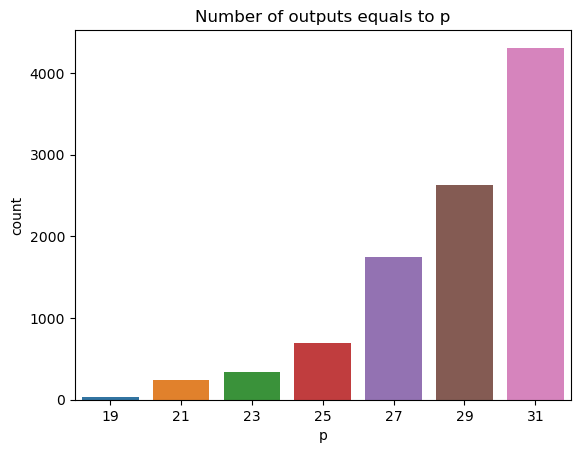
\includegraphics[width=\linewidth]{img/p_encodings/heuristic_ascon_0_p_frequencies.png}
    \caption{The outputs of $10000$ runs of the Algorithm \ref{alg:heuristic_matthieu} for the first subfunction of the Ascon s-box}
    \label{fig:ascon_0_p_frequencies}
  \end{minipage} \hfill
  \begin{minipage}{0.48\linewidth}
    \centering
    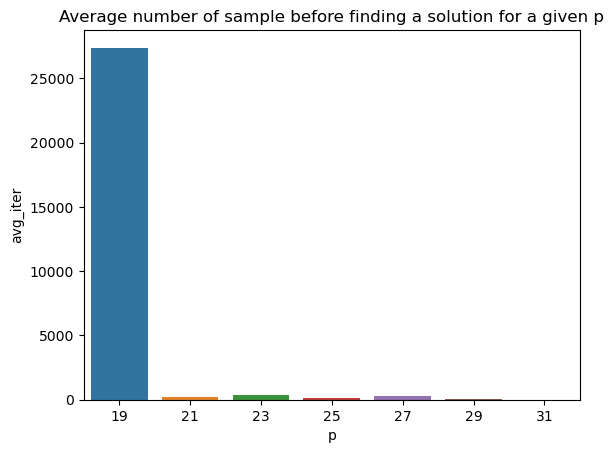
\includegraphics[width=\linewidth]{img/p_encodings/heuristric_ascon_0_count_iter.png}
    \caption{Number of iterations required to get a solution for a given value of $p$}
    \label{fig:ascon_0_count_iter}
  \end{minipage}
\end{figure}


In the process of finding the smallest $p$ possible and a correct vector of $p$-encoding to evaluate a function $f$, this heuristic is really efficient to get a tight upper bound on the value of $p$.

